\documentclass[border=6pt]{standalone}
\usepackage{tikz}
\usepackage{xcolor}
\usetikzlibrary{positioning,shapes.geometric,arrows.meta,calc,fit,backgrounds,decorations.pathmorphing}

\definecolor{naivered}{HTML}{E15759}
\definecolor{alignedblue}{HTML}{4E79A7}
\definecolor{readygreen}{HTML}{59A14F}
\definecolor{paneltint}{HTML}{F5F5F5}
\definecolor{cachegray}{HTML}{E8E8E8}

\begin{document}
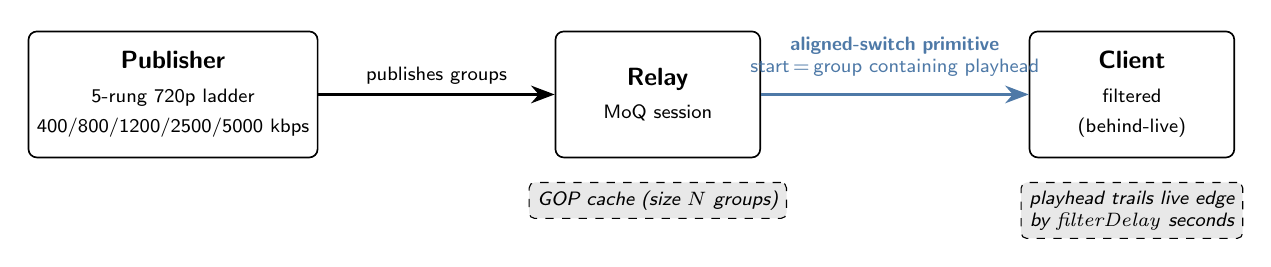
\begin{tikzpicture}[
  font=\sffamily\small,
  box/.style={
    draw, rounded corners=3pt,
    minimum width=26mm, minimum height=16mm,
    align=center, fill=white,
    line width=0.6pt,
    inner sep=3pt
  },
  inner/.style={
    draw, dashed, rounded corners=2pt,
    fill=cachegray, inner sep=3pt,
    align=center, font=\sffamily\scriptsize\itshape,
    line width=0.4pt
  },
  flow/.style={-{Stealth[length=3mm]}, line width=0.8pt},
]

% Three main nodes with extra horizontal space.
\node[box] (pub) {\textbf{Publisher}\\[1pt]\scriptsize 5-rung 720p ladder\\\scriptsize 400/800/1200/2500/5000 kbps};
\node[box, right=30mm of pub] (relay) {\textbf{Relay}\\[1pt]\scriptsize MoQ session};
\node[box, right=34mm of relay] (client) {\textbf{Client}\\[1pt]\scriptsize filtered\\\scriptsize (behind-live)};

% Inner annotations under each main node.
\node[inner, below=3mm of relay.south, anchor=north] (cache)
  {GOP cache (size $N$ groups)};
\node[inner, below=3mm of client.south, anchor=north] (lag)
  {playhead trails live edge\\by $\mathit{filterDelay}$ seconds};

% Pub -> Relay arrow with single-line label above.
\draw[flow] (pub) -- node[above, font=\sffamily\scriptsize, midway]
  {publishes groups} (relay);

% Relay -> Client arrow: label is a SINGLE compact node ABOVE the
% arrow midpoint so it doesn't bleed into the Client box.
\draw[flow, alignedblue] (relay.east) --
  node[above=1mm, midway, font=\sffamily\scriptsize, text=alignedblue, align=center]
       {\textbf{aligned-switch primitive}\\start\,$=$\,group containing playhead}
  (client.west);

\end{tikzpicture}
\end{document}
